% ------------------------------------------------------------------------------
% 7.1. DISEÑO DE LA ARQUITECTURA
% ------------------------------------------------------------------------------
\subsection{7.1. Diseño de la Arquitectura}\label{sec:cap7_arquitectura}

% [PENDIENTE]: Redactar la introducción del diseño de la arquitectura.

\subsubsection{7.1.1. Diseño Físico}\label{sec:cap7_diseno_fisico}

El diseño físico describe la arquitectura física del sistema, es decir, su topología: los nodos de hardware y los entornos de ejecución, junto con los artefactos de software que se ejecutan en cada uno y los protocolos de comunicación entre ellos. Se representa mediante un diagrama de despliegue del Lenguaje Unificado de Modelado \parencite{booch2005uml, rumbaugh2004uml}.

El sistema se organiza en tres grupos de nodos. El primero corresponde al cliente: la aplicación web (React y TypeScript), que se ejecuta en el navegador de una computadora personal, y la aplicación móvil (Flutter), que se ejecuta en un dispositivo Android y utiliza la cámara para digitalizar los documentos de la postulación. El segundo grupo corresponde a la nube de Amazon Web Services (AWS), que contiene un servidor de aplicación con Docker Engine, donde se ejecutan en contenedores separados la API REST (Java y Spring Boot, que emite y verifica los tokens JWT de autenticación) y el servicio de preselección en Python; un servidor de base de datos con PostgreSQL; y MinIO (almacenamiento de objetos compatible con S3) para el almacenamiento de los documentos adjuntos, las actas de adjudicación y las planillas de asistencia en formato PDF. El tercer grupo reúne los servicios externos de Firebase, de los cuales se emplea Firebase Cloud Messaging (FCM) para el envío de notificaciones \textit{push} al dispositivo móvil.

Las aplicaciones cliente se comunican con la API REST mediante HTTPS en formato JSON; el módulo de preselección solo es accesible desde la API, mediante una interfaz interna HTTP, y no se expone a los clientes. La API accede a PostgreSQL mediante JDBC, a MinIO mediante su API compatible con S3 y a FCM mediante el SDK de administración de Firebase. La Figura~\ref{fig:diagrama_despliegue} presenta el diagrama de despliegue general del sistema.

\begin{landscape}
\begin{figure}[p]
\caption{Diagrama de despliegue general del sistema}
\label{fig:diagrama_despliegue}
\centering
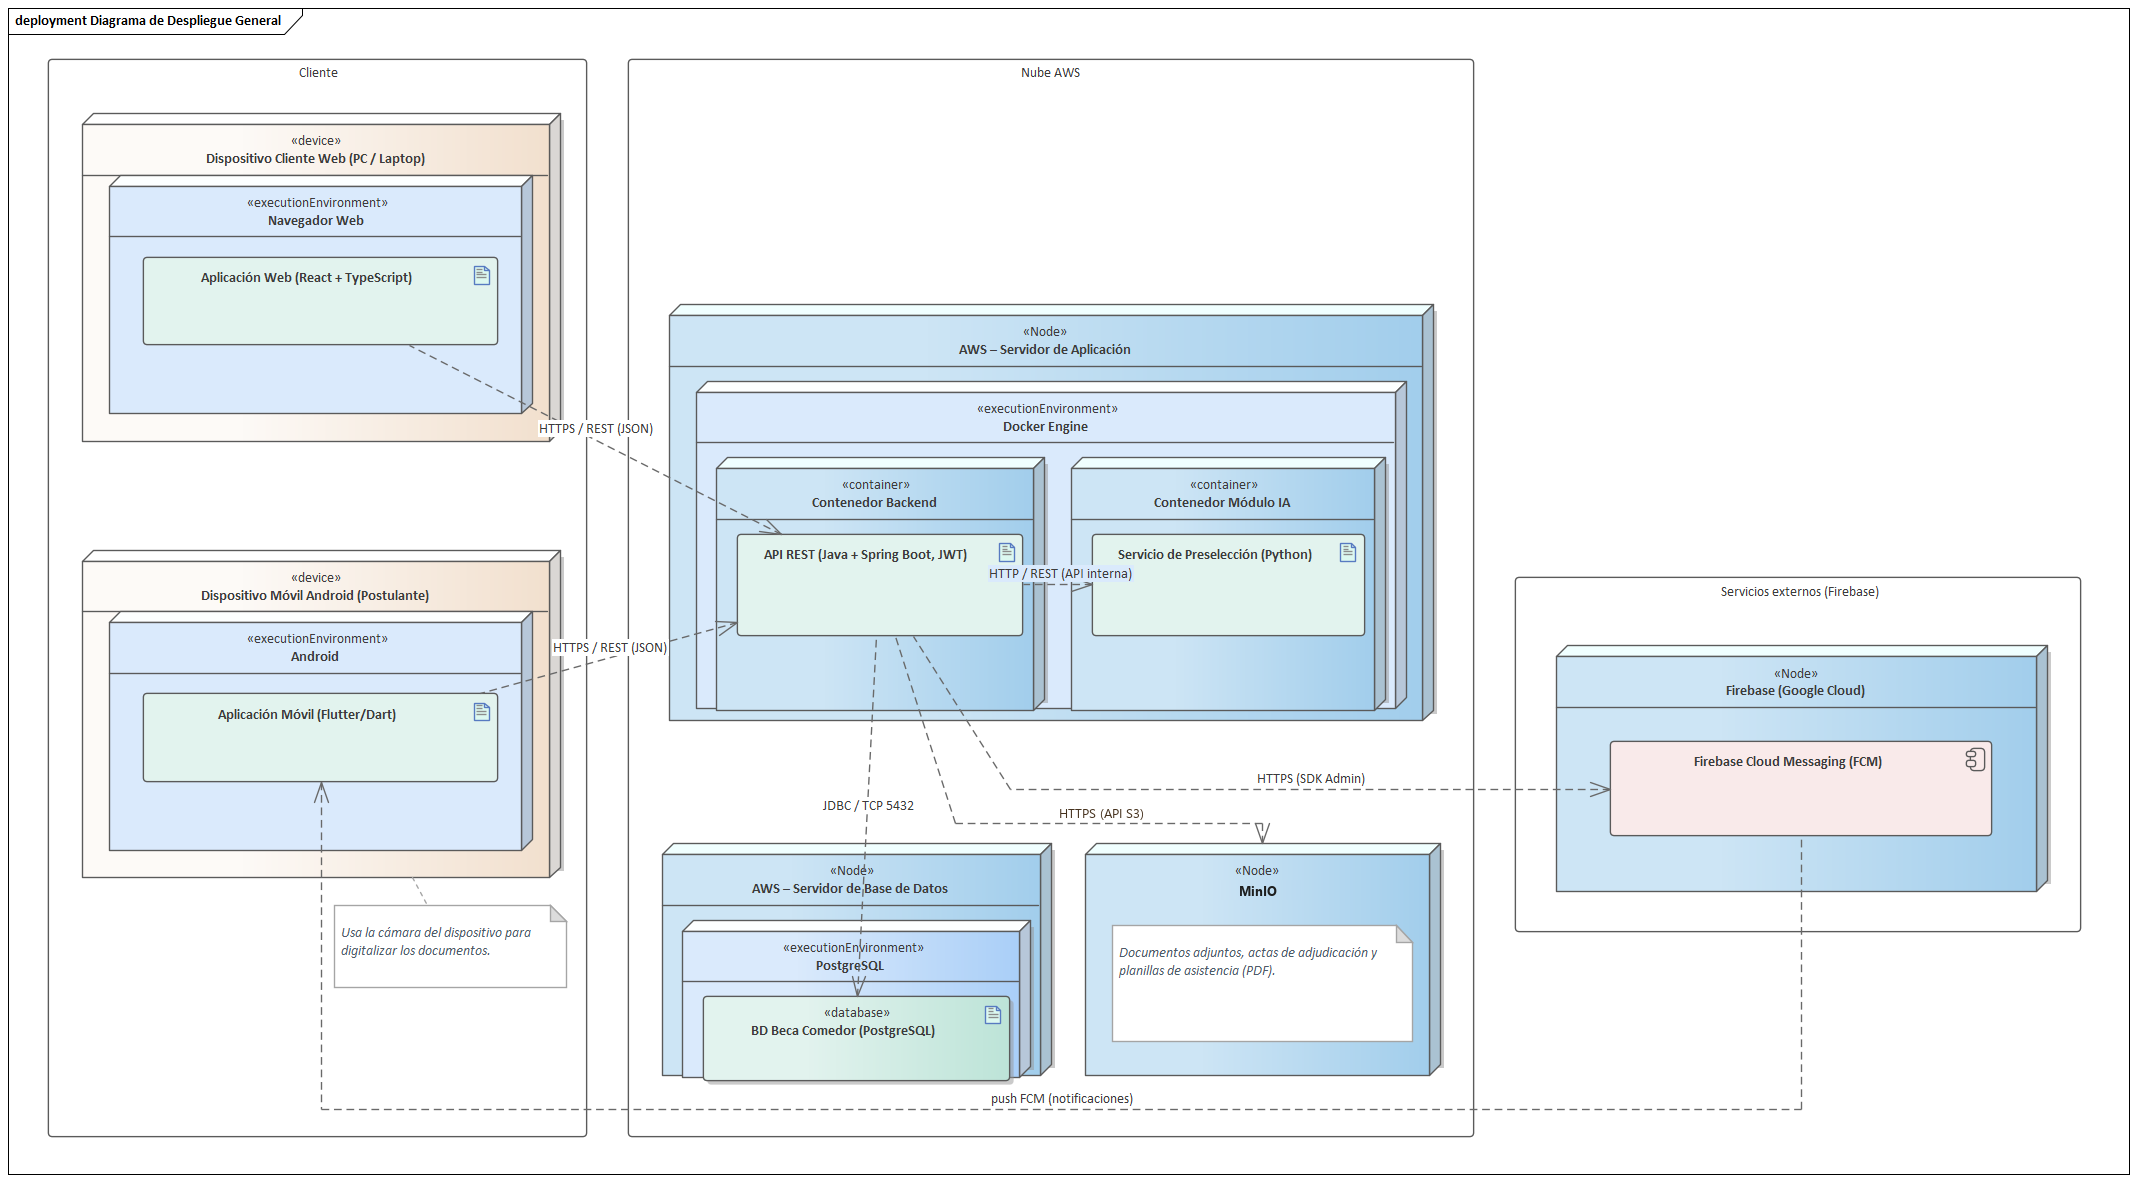
\includegraphics[width=\linewidth,height=0.8\textheight,keepaspectratio]{images/118_Diagrama_Despliegue_General.png}

\smallskip
\noindent\raggedright\textit{Nota.} Elaboración propia.
\end{figure}
\end{landscape}

\subsubsection{7.1.2. Diseño Lógico}\label{sec:cap7_diseno_logico}

El diseño lógico describe la organización interna del sistema en capas y paquetes, independientemente de los nodos físicos en los que se ejecuta (sección~\ref{sec:cap7_diseno_fisico}). Se representa mediante diagramas de paquetes del Lenguaje Unificado de Modelado, en los que cada capa agrupa los paquetes con responsabilidades afines y las dependencias de uso (\textit{use}) se dirigen de las capas superiores hacia las inferiores \parencite{booch2005uml, rumbaugh2004uml}. Este criterio es coherente con el encapsulamiento de los casos de uso en paquetes realizado en el análisis (sección~\ref{sec:cap6_encapsulamiento_cu}), de modo que los seis paquetes funcionales identificados se conservan como módulos de la capa de negocio \parencite{jacobson1999unified}.

\paragraph{Arquitectura lógica general.} La Figura~\ref{fig:diseno_logico_general} presenta la arquitectura lógica general del sistema, organizada en cuatro capas y un paquete de aspectos transversales. La capa de presentación contiene la aplicación web (React y TypeScript) y la aplicación móvil (Flutter), con las que interactúan los usuarios del sistema. La capa de servicios expone la API REST de Spring Boot, con sus controladores y objetos de transferencia de datos, y el mecanismo de autenticación y autorización, que emite y verifica los tokens JWT y aplica el rol del usuario. La capa de negocio agrupa los módulos de cuentas y acceso, convocatoria y postulación, auditoría y adjudicación, becados y asistencia, reportes y trazabilidad, y preselección con inteligencia artificial; este último se implementa en Python como servicio independiente que se consume mediante una API interna. La capa de acceso a datos reúne los repositorios (JPA e Hibernate) y los agentes de servicios externos, que a su vez dependen de la base de datos PostgreSQL y de los servicios externos (notificaciones push, almacenamiento de archivos y módulo de inteligencia artificial). Finalmente, los aspectos transversales (seguridad, bitácora y auditoría de acciones, manejo de errores y validaciones, y notificaciones) son utilizados por todas las capas.

\begin{landscape}
\begin{figure}[p]
\caption{Arquitectura lógica general del sistema en capas}
\label{fig:diseno_logico_general}
\centering
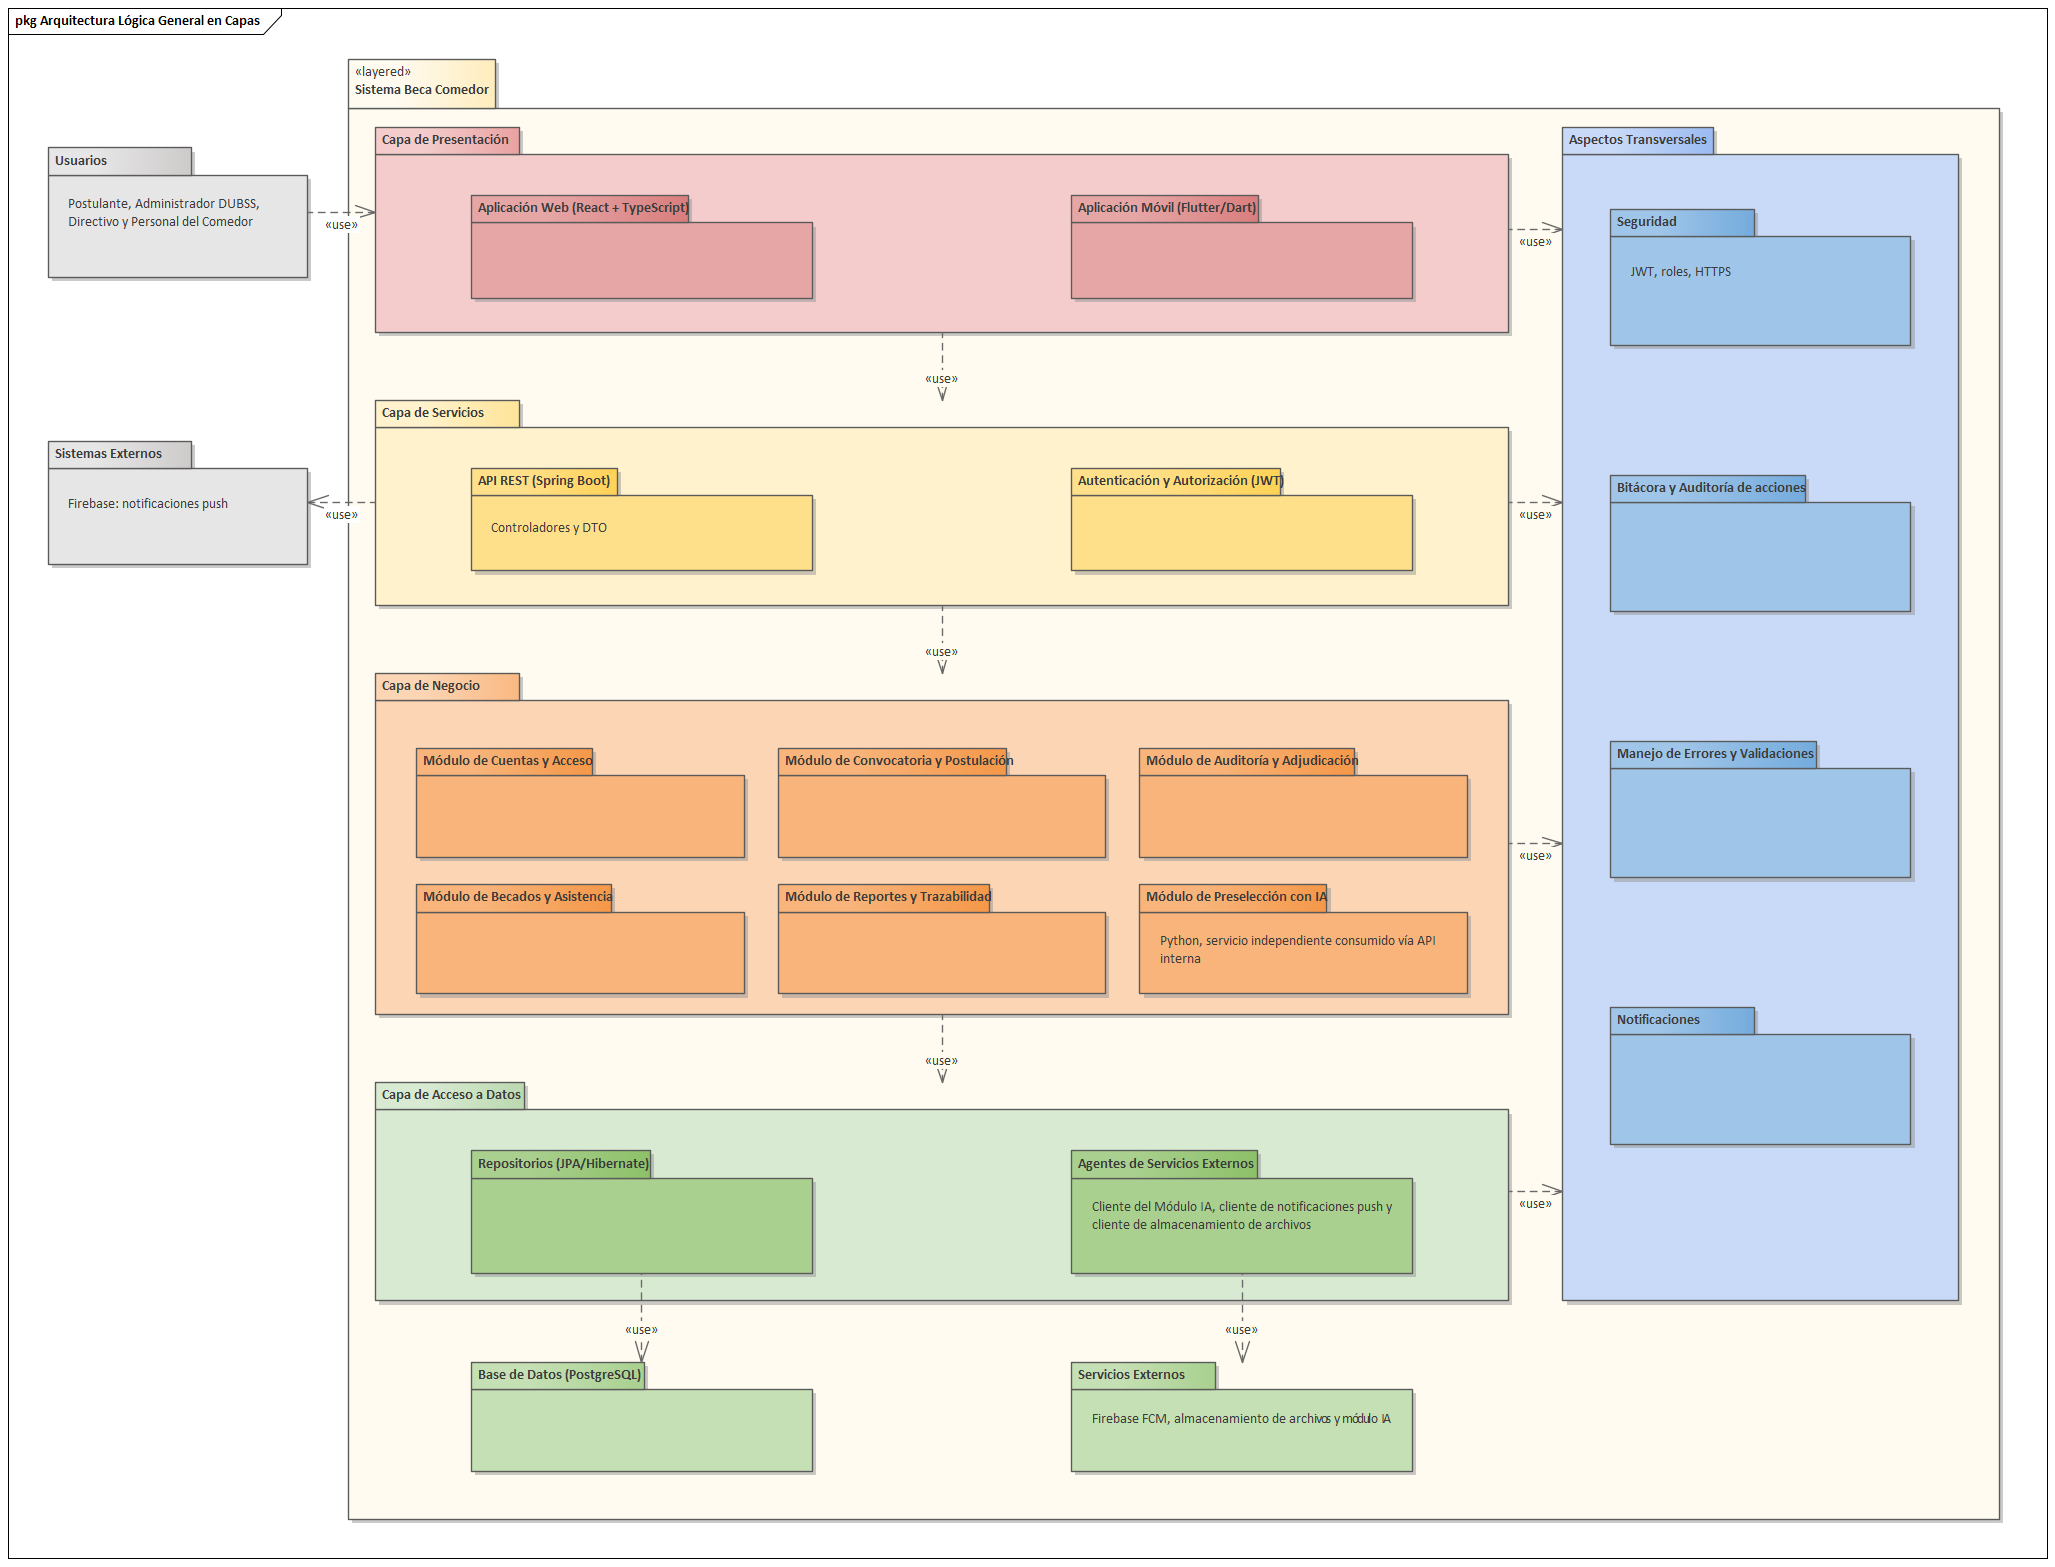
\includegraphics[width=\linewidth,height=0.8\textheight,keepaspectratio]{images/119_Diseno_Logico_Arquitectura_General.png}

\smallskip
\noindent\raggedright\textit{Nota.} Elaboración propia.
\end{figure}
\end{landscape}

\paragraph{Arquitectura lógica del \textit{backend}.} La Figura~\ref{fig:diseno_logico_backend} detalla la organización del \textit{backend} desarrollado con Spring Boot. La capa de presentación (API) contiene los controladores REST y los objetos de transferencia de datos con sus mapeadores; los controladores invocan a los servicios de la capa de lógica de aplicación, que se organizan según los seis paquetes funcionales: cuentas y acceso (P1), convocatoria y postulación (P2), preselección con IA (P3), auditoría y adjudicación (P4), becados y asistencia (P5), y reportes y trazabilidad (P6). Entre estos paquetes existen dependencias que reflejan el flujo del proceso: los servicios de becados y asistencia utilizan los de auditoría y adjudicación, estos utilizan los de convocatoria y postulación, y estos últimos los de preselección con IA. Los servicios operan sobre la capa de dominio, que contiene las entidades y las enumeraciones (por ejemplo, el estado de la postulación), y acceden a la capa de persistencia, conformada por los repositorios JPA, el cliente del módulo de inteligencia artificial y los clientes de notificaciones push y de almacenamiento de archivos. Los repositorios acceden a la base de datos PostgreSQL, y el paquete de seguridad y bitácora es utilizado por todas las capas.

\begin{landscape}
\begin{figure}[p]
\caption{Arquitectura lógica del \textit{backend} (Spring Boot)}
\label{fig:diseno_logico_backend}
\centering
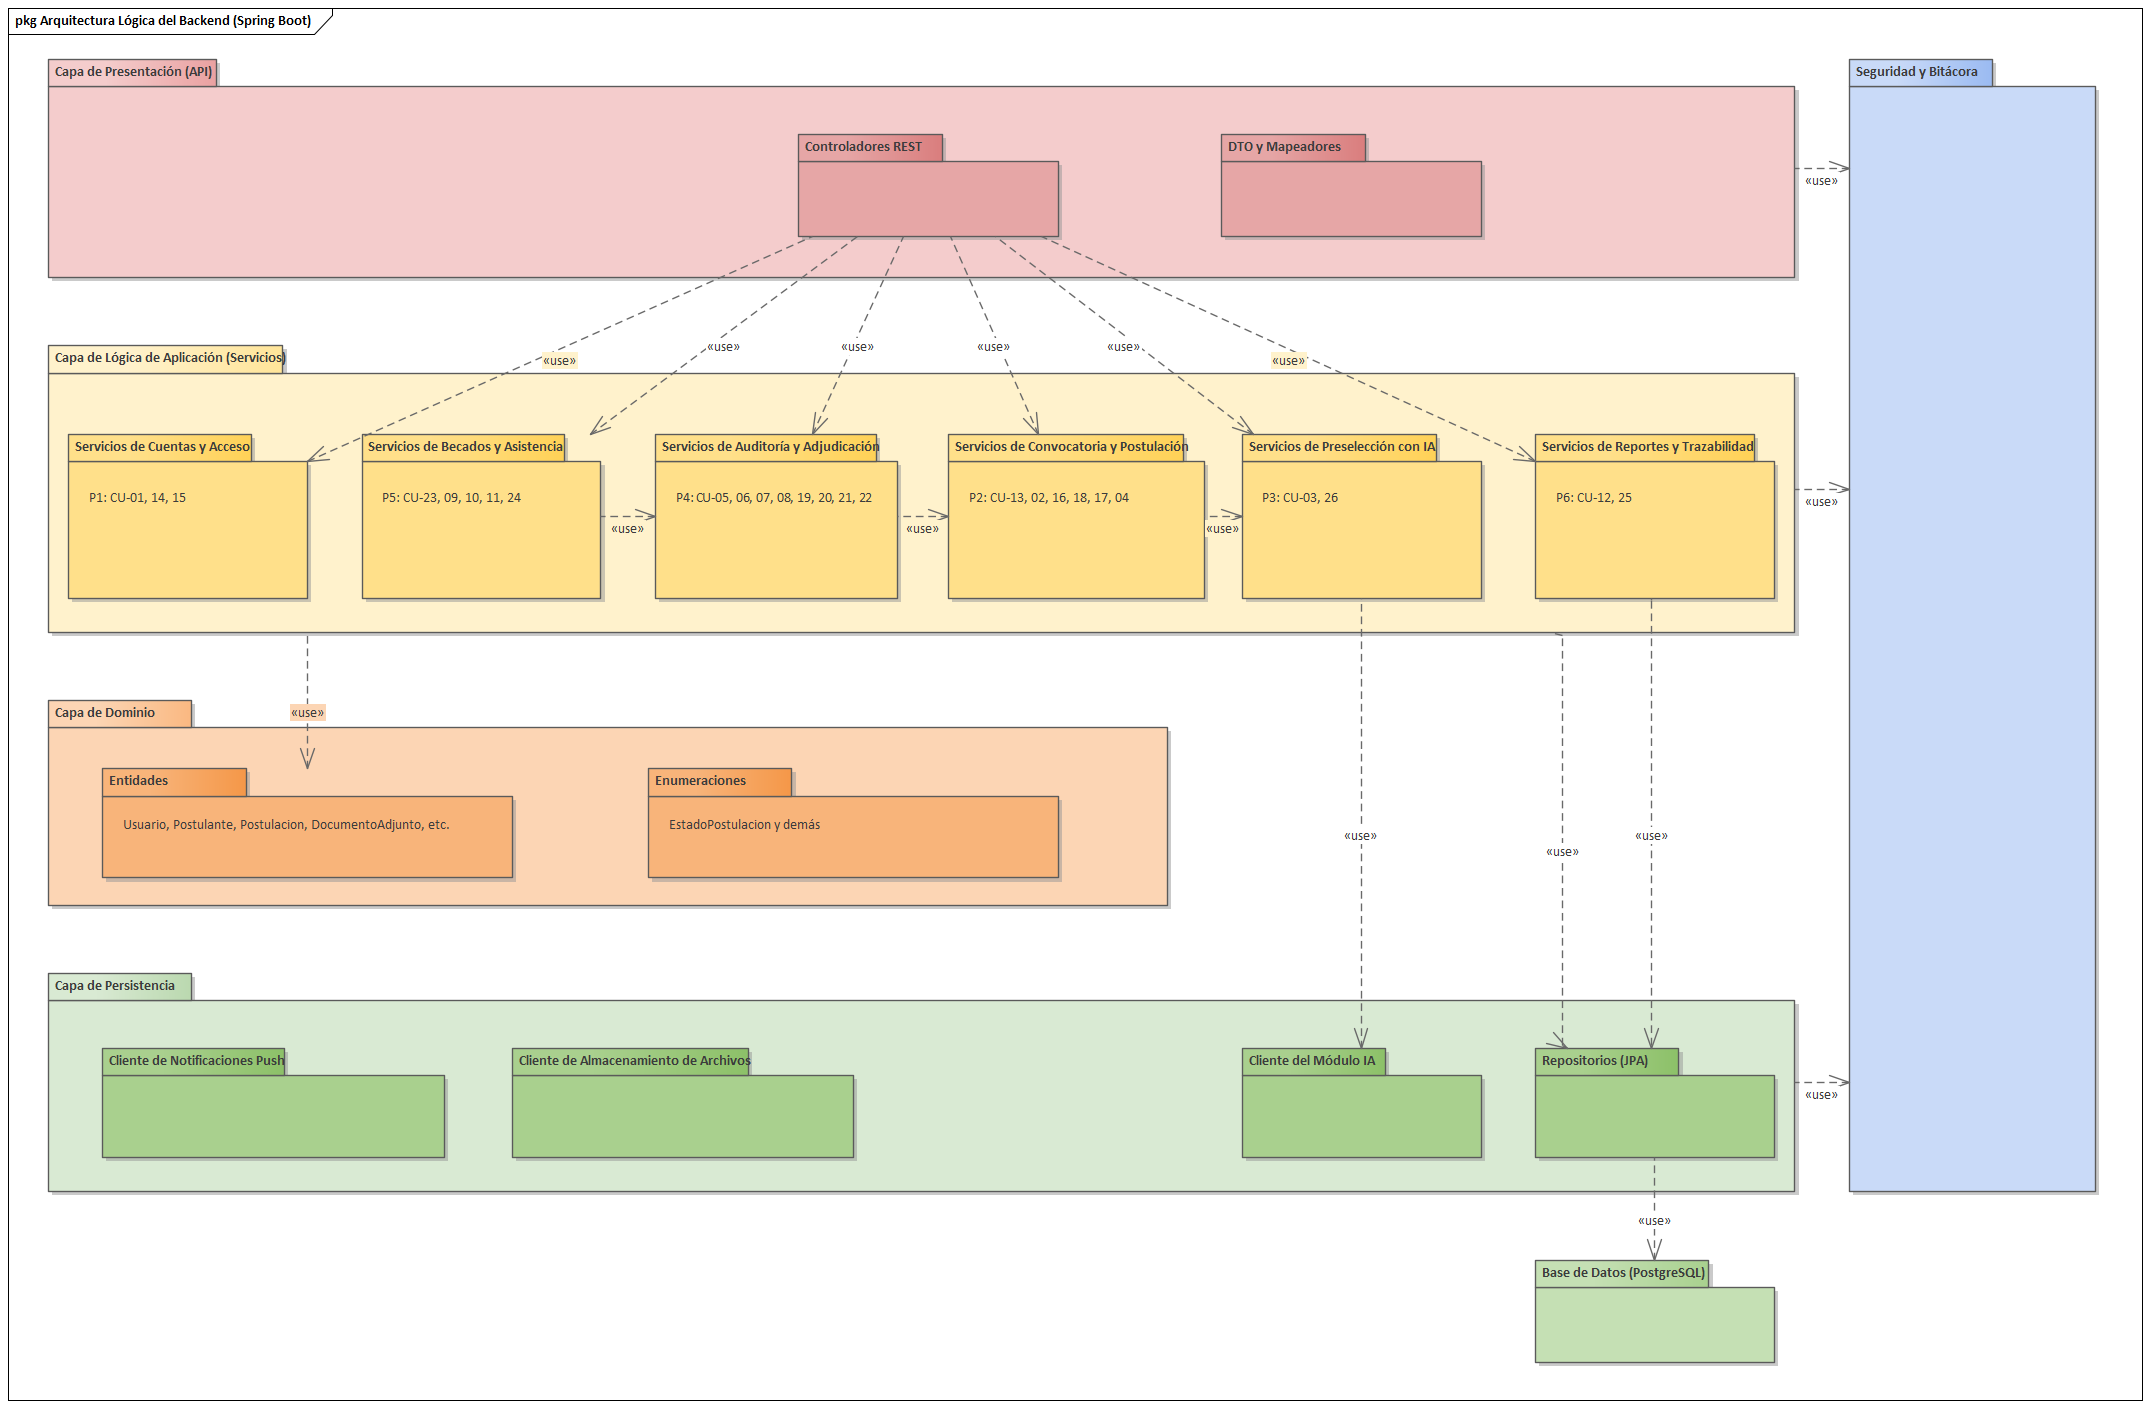
\includegraphics[width=\linewidth,height=0.8\textheight,keepaspectratio]{images/120_Diseno_Logico_Backend.png}

\smallskip
\noindent\raggedright\textit{Nota.} Elaboración propia. P1 a P6 corresponden a los paquetes de casos de uso definidos en el análisis.
\end{figure}
\end{landscape}
